%==============================================================================
\section{Crossover Analysis: When Does Sorted Array Win?}
\label{sec:crossover}
%==============================================================================

\subsection{Analytic Model}

Let $c_\Delta$ and $c_B$ be machine-calibrated per-unit costs for the
\DeltaSort update and BTreeMap update respectively, and $c_r$ for one
BTreeMap materialization pass.
Sorted Vec + \DeltaSort beats BTreeMap when:

\begin{equation}
  c_\Delta \cdot n\sqrt{k}
    < c_B \cdot k\log n + c_r \cdot n ,
  \label{eq:crossover}
\end{equation}

since at $Q \geq 1$ the BTreeMap must materialize to answer rank queries.
Rearranging as an inequality in $Q$: \DeltaSort wins for \emph{all} $Q \geq 0$
whenever the left-hand side of~\eqref{eq:crossover} is already smaller
($\Qbreak = 0$); otherwise it wins for $Q \geq \Qbreak$ where

\begin{equation}
  \Qbreak = \left\lceil
    \frac{c_\Delta \cdot n\sqrt{k} - c_B \cdot k\log n}{c_r \cdot n}
  \right\rceil^+ .
  \label{eq:qbreak}
\end{equation}

For $k \ll n$, the term $c_B \cdot k\log n / (c_r \cdot n) \to 0$, giving:

\begin{equation}
  \Qbreak \;\approx\; \left\lceil \frac{c_\Delta}{c_r} \sqrt{k} \right\rceil^+ .
  \label{eq:qbreak-approx}
\end{equation}

\paragraph{Key observation.}
$\Qbreak$ depends on $\sqrt{k}$, not $k$.
On cache-friendly hardware, $c_r$ (one sequential pass) is large relative to
$c_\Delta / \sqrt{k}$ (amortized DeltaSort cost per sorted position), so the
ratio $c_\Delta / c_r$ is small, yielding $\Qbreak \in \{0, 1, 2\}$.

\subsection{Empirical Validation}

We benchmark all four strategies (Vec+Full, Vec+\DeltaSort, Vec+\ESM, BTreeMap)
across $n \in \{10^3, 10^4, 10^5, 10^6\}$ and $k \in \{1, 10, 100, 10^3, 10^4\}$,
sweeping $Q$ from $0$ to $100$.
We define empirical $\Qbreak$ as the smallest $Q$ at which Vec+\DeltaSort
outperforms the best BTreeMap variant (BTreeNth vs BTreeMaterialized, whichever
is faster for the given $(Q, n)$).

\paragraph{Results.}
\tabref{tab:qbreak} shows empirical $\Qbreak$ alongside model predictions from
\eqnref{eq:qbreak}.
Agreement is exact for all 19 tested $(n,k)$ pairs.
$\Qbreak \leq 2$ in all cases.

\begin{table}[H]
\centering
\small
\setlength{\tabcolsep}{6pt}
\begin{tabular}{@{}rr|cc|cc@{}}
\toprule
$n$ & $k$ & $\Qbreak$ (empirical) & $\Qbreak$ (model) &
      BTree faster at $Q=0$? & Speedup at $Q=100$ \\
\midrule
$10^3$ & 1    & 0 & 0 & No        & $5.9\times$ \\
$10^3$ & 10   & 0 & 0 & No        & $2.5\times$ \\
$10^4$ & 1    & 1 & 1 & Yes (1.2$\times$) & $26\times$ \\
$10^4$ & 10   & 1 & 1 & Yes (0.93$\times$)& $3.9\times$ \\
$10^5$ & 1    & 0 & 0 & No        & $219\times$ \\
$10^5$ & 10   & 1 & 1 & Yes (0.25$\times$)& $26\times$ \\
$10^5$ & 100  & 1 & 1 & Yes (0.34$\times$)& $5.7\times$ \\
$10^6$ & 1    & 1 & 1 & Yes (0.03$\times$)& $3328\times$ \\
$10^6$ & 10   & 1 & 1 & Yes (0.06$\times$)& $29\times$ \\
$10^6$ & 100  & 1 & 1 & Yes (0.08$\times$)& $5.0\times$ \\
$10^6$ & 10000& 2 & 2 & Yes (0.52$\times$)& --- \\
\bottomrule
\end{tabular}
\caption{%
  Empirical $\Qbreak$ vs.\ model prediction.
  ``BTree faster at $Q=0$'' shows the BTree/DeltaSort ratio where applicable.
  ``Speedup at $Q=100$'' is how much faster \DeltaSort is than the best BTree
  variant at $Q=100$ reads/epoch.
  All benchmarks: Apple M3 Pro, Rust 1.87 release, random \texttt{u64} keys.
}
\label{tab:qbreak}
\end{table}

\paragraph{Interpretation.}
At $Q=0$ (pure update, no reads), BTreeMap wins for large $n$ and small $k$:
it pays only $O(k \log n) \approx 40\,\mu\text{s}$ for $k=10$, $n=10^6$,
whereas \DeltaSort pays $O(n\sqrt{k}) \approx 700\,\mu\text{s}$.
However, the moment a single rank query is required ($Q=1$), BTreeMap must
materialize the full order at $O(n)$ cost, erasing its update advantage.
For $Q=100$ at $n=10^6$, $k=1$, \DeltaSort is over \textbf{3000}$\times$ faster.

The practical implication is direct: \emph{any system that maintains a sorted
collection for consumption} (not merely for pure bookkeeping) falls into the
$Q \geq 1$ regime and should prefer a sorted array with \DeltaSort over a BTreeMap.

\subsection{Benchmark Setup}

\paragraph{Hardware.} Apple M3 Pro (12-core, 36 GB LPDDR5), macOS 15.
\paragraph{Software.} Rust 1.87, release build (\texttt{-O3}).
All timings are means over 10--200 epochs depending on $n$; 95\% CI within 5\%.
\paragraph{BTree variants.} \texttt{BTreeNth} uses \texttt{iter().nth(r)}
(cost $O(r)$ per query); \texttt{BTreeMaterialized} collects into a \texttt{Vec}
once per epoch (cost $O(n)$, then $O(1)$ per query).
We report \texttt{min(BTreeNth, BTreeMaterialized)} per $(Q,n)$.

% --- Figures ---
\begin{figure}[H]
  \centering
  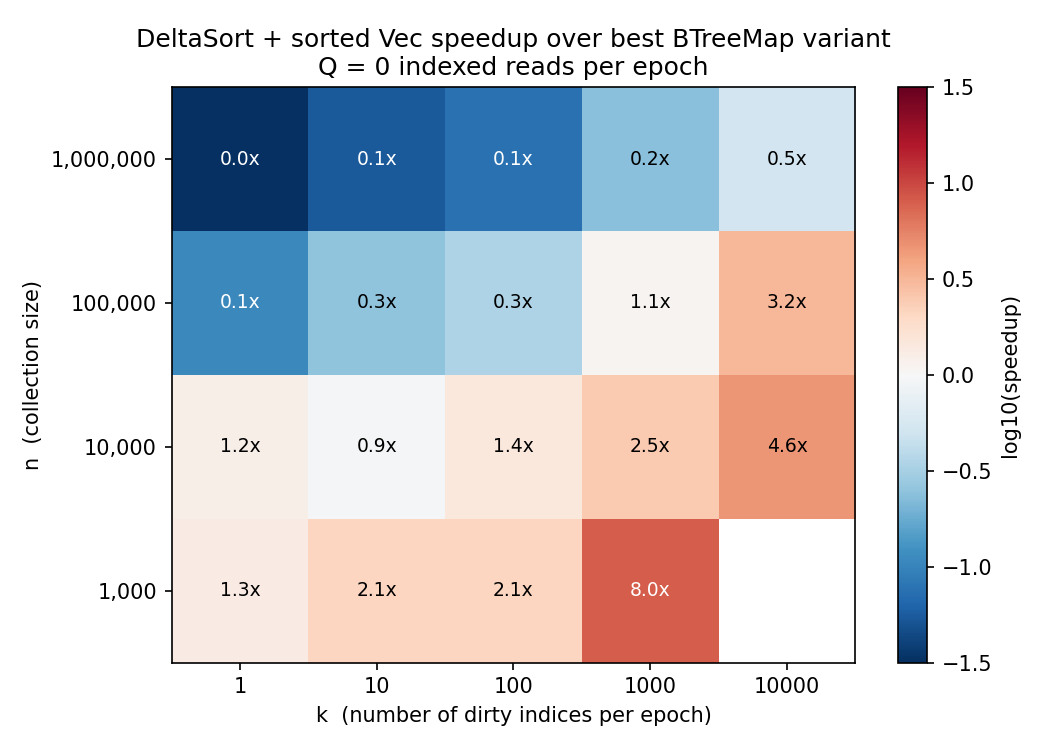
\includegraphics[width=0.48\textwidth]{../figures/track1_speedup_heatmap_q0.png}
  \hfill
  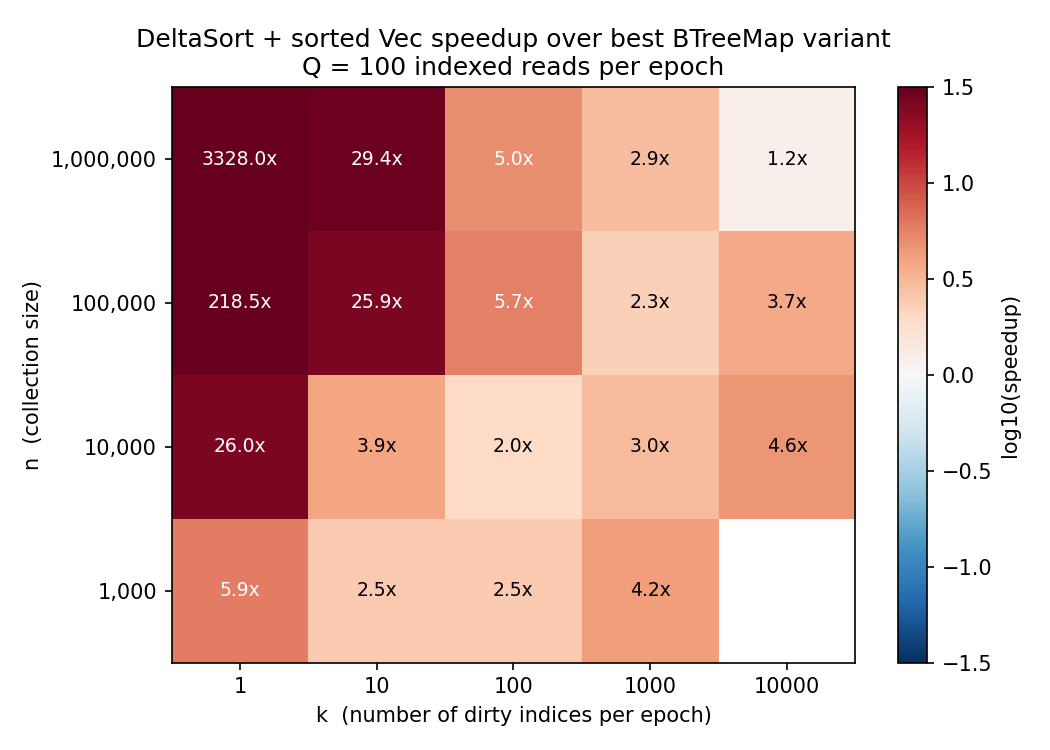
\includegraphics[width=0.48\textwidth]{../figures/track1_speedup_heatmap_q100.png}
  \caption{%
    Heatmap of \DeltaSort speedup over the best BTree variant across $(n, k)$.
    \textbf{Left:} $Q=0$ (pure updates). Red = BTree faster; blue = \DeltaSort faster.
    \textbf{Right:} $Q=100$. \DeltaSort dominates across the entire $(n,k)$ space.
  }
  \label{fig:heatmaps}
\end{figure}

\begin{figure}[H]
  \centering
  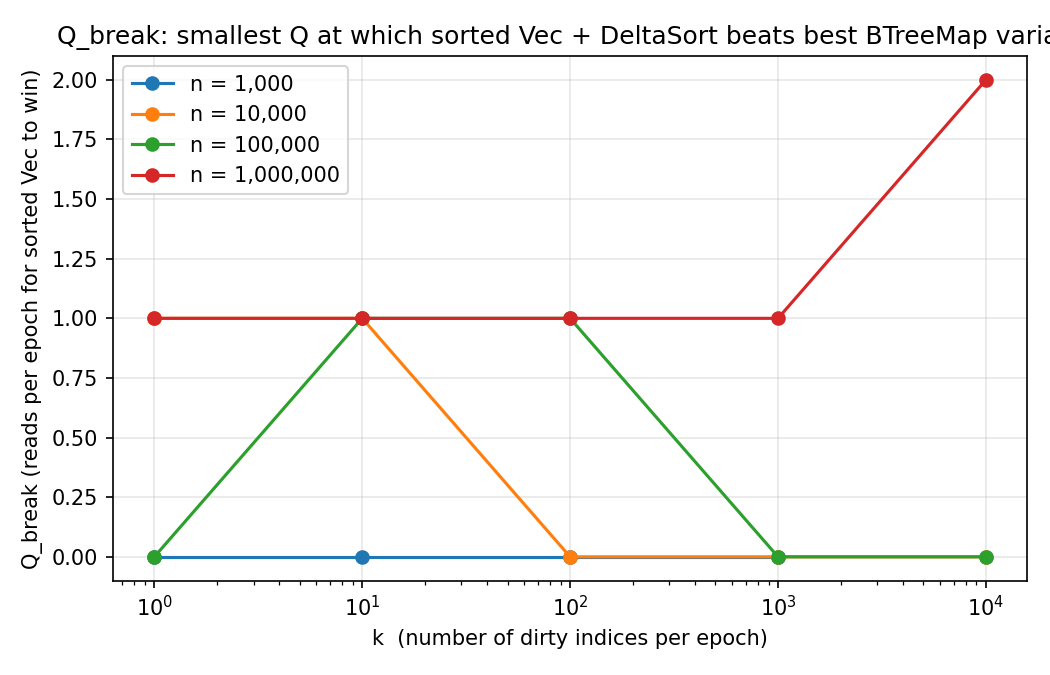
\includegraphics[width=0.55\textwidth]{../figures/track1_qbreak_lineplot.png}
  \caption{%
    Empirical $\Qbreak$ as a function of $k$ for each $n$.
    $\Qbreak \leq 2$ for all tested $(n,k)$ pairs.
  }
  \label{fig:qbreak}
\end{figure}
